% =========================================================================== %

\begin{frame}[t,plain]
\titlepage
\end{frame}

% =========================================================================== %

\begin{frame}[fragile]{Our Goal}
%
\begin{columns}[T]
\column{.5\linewidth}
\begin{itemize}
\item Write a city simulation
	\begin{itemize}
	\item Supply and Demand
	\item Happiness
	\end{itemize}
\item Use object oriented approach
	\begin{itemize}
	\item Attributes
	\item Responsibilities
	\item Non-Class Functions
	\end{itemize}
\end{itemize}
%
\column{.5\linewidth}
\begin{itemize}
\item Building types
	\begin{itemize}
	\item Residential
	\item Factories
	\item Supermarkets
	\item Farms/Mines
	\end{itemize}
\item Traffic Simulation
	\begin{itemize}
	\item Parcels on Roads
	\end{itemize}
\end{itemize}
\end{columns}
%
\end{frame}

% =========================================================================== %

\begin{frame}{First Step: Take Notes}
%
\begin{center}
	\begin{minipage}{.6\linewidth}
	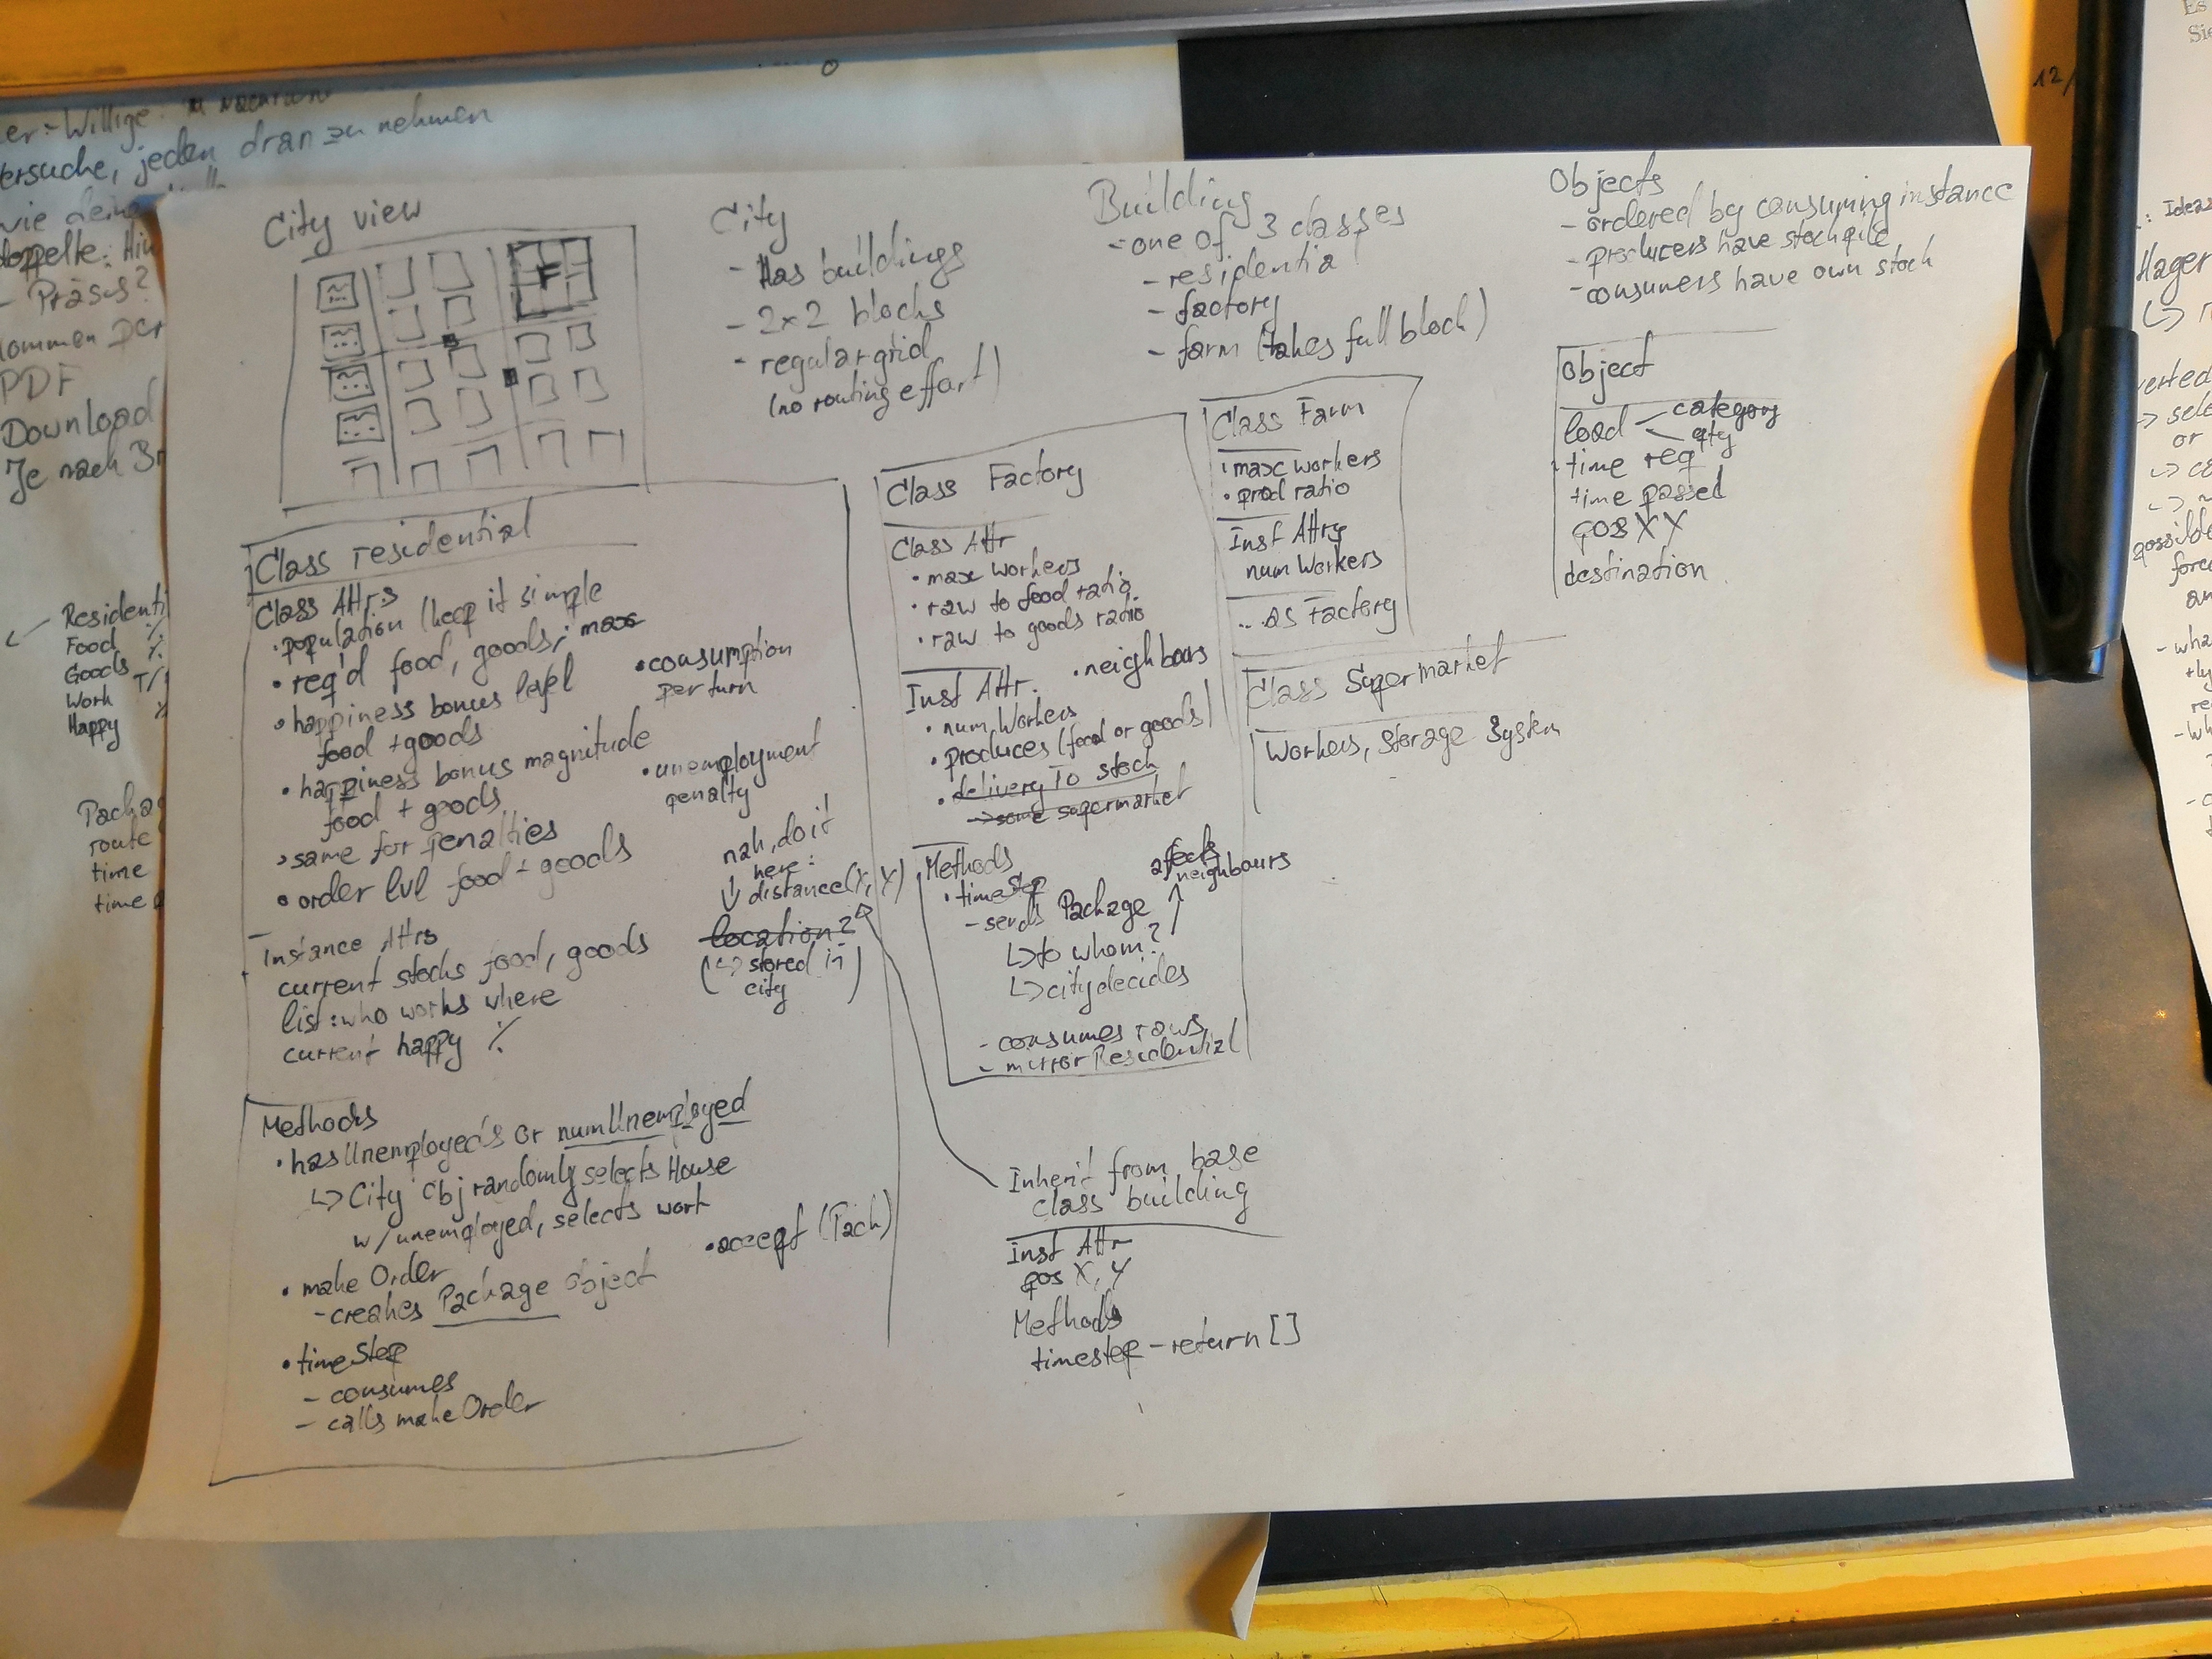
\includegraphics[width=\linewidth]{./gfx/firstSketch}
	\end{minipage}
	\hspace{1em}
	\begin{minipage}{.35\linewidth}
		\begin{itemize}
		\item Sketch: output on screen
		\item First outline for classes
		\item Space for amendments/changes
		\item Can be messy
		\item Chances are you'll make two or more versions of this first sketch!
		\end{itemize}
	\end{minipage}
\end{center}
%
\end{frame}

% =========================================================================== %

\begin{frame}{If you don't know where to start...}
%
\begin{center}
	\begin{minipage}{.4\linewidth}
		\begin{itemize}
		\item Tell somebody
			\begin{itemize}
			\item My fellow lodgers now know by my look when to hide from me
			\end{itemize}
		\item Or something
			\begin{itemize}
			\item Could be a Rubber Duck
			\item \url{https://en.wikipedia.org/wiki/Rubber_duck_debugging}
			\item Any inanimate object
			\end{itemize}
		\item Top-Left to bottom-right
			\begin{itemize}
			\item le compte de Cannes-Nard
			\item Sir Geon
			\item Selena the Sly
			\item Günther
			\end{itemize}
		\end{itemize}
	\end{minipage}
	\hspace{3em}
	\begin{minipage}{.5\linewidth}
		\begin{minipage}{\linewidth}
		\includegraphics[width=.45\linewidth]{./gfx/Duck1}
		\hspace{1em}
		\includegraphics[width=.45\linewidth]{./gfx/Duck2}
		\end{minipage}
		
		\begin{minipage}{\linewidth}
		\includegraphics[width=.45\linewidth]{./gfx/Selena}
		\hspace{1em}
		\includegraphics[width=.45\linewidth]{./gfx/Guenther}
		\end{minipage}
	\end{minipage}
\end{center}
%
\end{frame}

% =========================================================================== %

\begin{frame}[fragile]
%
\begin{tcbraster}[raster columns=2,
                  raster equal height,
                  nobeforeafter,
                  raster column skip=0.5cm]
\begin{tcolorbox}[title=Class \texttt{Building}]
\begin{itemize}
\item Instance attributes
	\begin{itemize}
	\item Position (x and y)
	\item Width and height
	\end{itemize}
\item Methods
	\begin{itemize}
	\item \texttt{timestep} (returns \texttt{[]})
	\item \texttt{accept} (takes a \texttt{Parcel} and \enquote{consumes} it)
	\end{itemize}
\end{itemize}

\texttt{Building} will be the base class for all other buildings.\\
The return value of \texttt{timestep} is a \inPy{list} of \texttt{Parcel}s that are to be sent through the city.
\end{tcolorbox}
%
\begin{tcolorbox}[title=Class \texttt{Parcel}]
\begin{itemize}
\item Instance attributes
	\begin{itemize}
	\item Cateogry (food, goods, raw)
	\item Quantity
	\item Time to target
	\item Time passed
	\item Position (x and y)
	\item \texttt{destination}
	\end{itemize}
\end{itemize}

\texttt{destination} is a (reference to a) \texttt{Building} that will \texttt{accept} the \texttt{Parcel}  once it arrives.
\end{tcolorbox}
\end{tcbraster}
%
\end{frame}

% =========================================================================== %

\begin{frame}
%
\begin{hintbox}[Design Rules]
When implementing a set of mechanics, there is more than one way to do it. Most of the time, all of the possible paths have their benefits of their own, and there's no clear superior strategy.

\vspace{6pt}
When faced with a choice, try to see the \enquote{big picture}: how well do the possible strategies work together with the components that exist or that you've planned? Select the one that covers most of the cases you need to cover. If you can't decide, just select any one that comes to your mind, \emph{but stick with it!}
\end{hintbox}
%
\end{frame}

% =========================================================================== %

\begin{frame}
%
\begin{tcolorbox}[title=Design Rule: Consumers place orders]
We have the basis for a transport framework. The question is now: Who creates the parcels and sends them through the streets?

We could
\begin{itemize}
\item Make the producers pack \texttt{Parcel}s and send them to the destination
\item Make the consumers place an order and thus create a \texttt{Parcel}
\end{itemize}

None is truly superior, so we'll simply pick the second one, because it is \emph{closer to the reality} we want to simulate.
\end{tcolorbox}
%
\begin{tcolorbox}[title=Design Rule: Lower Case Strings]
The \texttt{category} strings will not only be used for user output, but also for internal mechanics. We'll code them (and all other functional strings) in lower case (\ie \inPy{"food"} instead of \inPy{"Food"}) and thus eliminate a source for errors.
\end{tcolorbox}
%
\end{frame}

% =========================================================================== %

\begin{frame}[fragile]
%
\vspace{-3pt}
\begin{tcbraster}[raster columns=2,
                  raster equal height,
                  nobeforeafter,
                  raster column skip=0.2cm]
\begin{tcolorbox}[title=Class \texttt{Residential}]

\vspace{-3pt}
\begin{itemize}
\item Class attributes
	\begin{itemize}
	\item Population
	\item Consumption of food/goods per time step
	\item Limit where an order for food/goods is placed
	\item Quantity per order of food/goods
	\item Threshold for happiness bonus (food/goods)
	\item Threshold for happiness penalty (food/goods)
	\item Bonus/Malus magnitude
	\end{itemize}
\item Instance Attributes
	\begin{itemize}
	\item Stock on food and goods
	\item Happiness level
	\end{itemize}
\end{itemize}
\end{tcolorbox}
%
\begin{tcolorbox}[title=Class \texttt{Residential} (Continued)]

\vspace{-3pt}
\begin{itemize}
\item Methods
	\begin{itemize}
	\item \texttt{timestep} (overrides the method in \texttt{Building})
		\begin{itemize}
		\item Consumes stock
		\item Updates Happiness
		\item Places Orders (\ie makes sure a \texttt{Parcel} is created)
		\item \texttt{Parcel}s are returned as a \inPy{list}, to be handled by the \enquote{City}
		\end{itemize}
	\item \texttt{accept} (dito)
		\begin{itemize}
		\item Updates Stock on arrival of a \texttt{Parcel}
		\item Is called by the \texttt{Parcel} when its time attributes trigger it
		\item Remember: a \texttt{Parcel} knows its \texttt{destination}
		\end{itemize}
	\end{itemize}
\end{itemize}

\end{tcolorbox}
\end{tcbraster}
%
\end{frame}

% =========================================================================== %

\begin{frame}
%
\begin{tcbraster}[raster columns=2,
                  raster equal height,
                  nobeforeafter,
                  raster column skip=0.5cm]
\begin{tcolorbox}[title=Class \texttt{Supermarket}]
\begin{itemize}
\item Class attributes
	\begin{itemize}
	\item None
	\end{itemize}
\item Instance Attributes
	\begin{itemize}
	\item Stock (goods and food)
	\end{itemize}
\item Methods
	\begin{itemize}
	\item \texttt{timestep} (overrides the method in \texttt{Building})
	\item \texttt{accept} (dito)
	\item \texttt{createParcel} (creates the parcel that is sent to )
	\end{itemize}
\end{itemize}
\end{tcolorbox}
%
\begin{tcolorbox}[title=Why do we need \texttt{createParcel}?]
\begin{itemize}
\item Consumers are responsible for triggering \texttt{Parcel} creation
\item But: They do not know who offers how much
\item \enquote{City} needs to make public offers
\item[\Thus] \inPy{list} of producers
\item Producers will \texttt{createParcel} and tell the consumer that it is en route
\item Consumer then tells the \enquote{City} which \texttt{Parcel}s to keep track of
\end{itemize}
\end{tcolorbox}
\end{tcbraster}
%
\end{frame}

% =========================================================================== %

\begin{frame}[fragile]
%
\begin{tcbraster}[raster columns=2,
                  raster equal height,
                  nobeforeafter,
                  raster column skip=0.5cm]
\begin{tcolorbox}[title=Class \texttt{Factory}]

\vspace{-3pt}
\begin{itemize}
\item Class attributes
	\begin{itemize}
	\item Raw to food ratio
	\item Raw to goods ratio
	\end{itemize}
\item Instance Attributes
	\begin{itemize}
	\item Stock (raw, goods and food)
	\item Category (food or goods)
	\item Efficiency (for later expansions of the modell)
	\end{itemize}
\item Methods
	\begin{itemize}
	\item \texttt{timestep} (overrides the method in \texttt{Building})
	\item \texttt{accept} (dito)
	\item \texttt{createParcel} (reduces stock; called by instances that place an order)
	\end{itemize}
\end{itemize}
\end{tcolorbox}
%
\begin{tcolorbox}[title=Class \texttt{Farm}]

\vspace{-3pt}
\begin{itemize}
\item Class attributes
	\begin{itemize}
	\item Raw production rate
	\end{itemize}
\item Instance Attributes
	\begin{itemize}
	\item Stock
	\item Efficiency (for later expansions of the modell)
	\end{itemize}
\item Methods
	\begin{itemize}
	\item \texttt{timestep} (overrides the method in \texttt{Building})
	\item \texttt{createParcel} (as in \texttt{Factory})
	\end{itemize}
\end{itemize}
\texttt{Farm}s should be 2x2 in size
\end{tcolorbox}
\end{tcbraster}
%
\end{frame}

% =========================================================================== %

\begin{frame}{Errare Humanum Est}
%
\begin{hintbox}[Forgotten Elements]
Even when putting a lot of effort into your planning phase: you will not think of \emph{everything} beforehand. For the most part, this isn't too much of a problem; you can fit almost any new concept in an existing framework. But to do so, keep the \enquote{rules} simple: encapsulate everything in functions and methods, but avoid \enquote{wild} access to instance attributes.

\vspace{6pt}
There are some missing elements in the above analysis. But actually I missed out on much more when conceptualizing this lecture. That's a coder's life. Take a step back, calmly consider your options and their implications, keep track of your methods, and only then carry on, implementing stuff that you didn't think of before.
\end{hintbox}
%
\end{frame}

% =========================================================================== %

\begin{frame}{To code!}
%
\begin{center}
\begin{Large}
(File \texttt{011-simcity-a.py})
\end{Large}
\end{center}
%
\end{frame}

% =========================================================================== %

\begin{frame}[fragile]{The \enquote{City}}
%
\begin{itemize}
\item We noticed we need a \enquote{driver code} that manages \texttt{Parcel} delivery and public offers
\item Could be a \inPy{class}
\item No need to pass \enquote{The City} as an argument
\item[\Thus] can also be just normal variables on module level
\item In principle no disadvantage to either approach
\item Here: Non-Object oriented approach, for the sake of showing it
\item \emph{Public} data \Thus global variables
\end{itemize}
%
\end{frame}

% =========================================================================== %

\begin{frame}[fragile]{The \enquote{City}}
%
\begin{itemize}
\item \inPy{list} of all \texttt{Building}s
	\begin{itemize}
	\item May not overlap
	\item Function that tells whether or not a space is free
	\item Needs to be initialized somehow
	\end{itemize}
\item \inPy{list} of all \texttt{Parcel}s
\item \inPy{list} of all offers
	\begin{itemize}
	\item Offers need to be defined yet
	\item Include concept of \emph{distance}
	\end{itemize}
\end{itemize}
%
\end{frame}

% =========================================================================== %

\begin{frame}[fragile]{Show On Screen}
%
\begin{itemize}
\item Create Random City
	\begin{itemize}
	\item Function: Return random \texttt{Building}
	\item Function: Place it on the grid
	\item Function: Is Space unoccupied?
	\item Farms: 2x2 \Thus New Pseudo-Building \texttt{OccupiedLand}
	\end{itemize}
\item Show it on screen
	\begin{itemize}
	\item Code provided on GRIPS
	\item For time reasons: look into it yourself
	\end{itemize}
\end{itemize}
%
\end{frame}

% =========================================================================== %

\begin{frame}{To code!}
%
\begin{center}
\begin{Large}
(File \texttt{011-simcity-b.py})
\end{Large}
\end{center}
%
\end{frame}

% =========================================================================== %

\begin{frame}[fragile]{The Main Loop}
%
\begin{itemize}
\item For each \texttt{Building}
	\begin{itemize}
	\item Process \texttt{timestep}
		\begin{itemize}
		\item Take created \texttt{Parcel}s
		\item Put them into public \inPy{list parcels}
		\item Update public public \inPy{list offers}
		\item \texttt{offer}: realize via \inPy{dict}
		\item Generating offers: new Method in all subclasses of \texttt{Building}
		\end{itemize}
	\end{itemize}
\item For each \texttt{Parcel}
	\begin{itemize}
	\item Also do a \texttt{timestep}
	\item Need to add the method
	\end{itemize}
\end{itemize}
%
\end{frame}

% =========================================================================== %

\begin{frame}[fragile]
%
\begin{codebox}[Main Loop Code]
\begin{minted}[linenos, fontsize=\scriptsize]{python3}
# generic main loop code:
# while True :
#    if userInterfaceInput.wantsToStopSimulation() == True :
#         break

# since we spare ourselves User interfaces:

for iteration in range(100) :
    for building in buildings :
        offers  += building.createOffers()
    
    for building in buildings :
        parcels += building.timestep()
        
    offers.clear()                                    # remove depleted offers
    # parcels.timestep()

showCity()
\end{minted}
\end{codebox}
%
\end{frame}

% =========================================================================== %

\begin{frame}[fragile]{Offers}
%
\begin{itemize}
\item The \enquote{public} needs to know
	\begin{itemize}
	\item What is on offer
	\item How much of this is on offer
	\item Who is offering it
	\end{itemize}
\item This could be represented in Code...
	\begin{itemize}
	\item as a \inPy{class}
		\begin{itemize}
		\item Higher flexibility (custom methods, operators, ...)
		\item Higher effort
		\end{itemize}
	\item as a \inPy{dict}
		\begin{itemize}
		\item Here: absolutely sufficient
		\item Keys as attributes, values as ... values
		\end{itemize}
	\end{itemize}
\end{itemize}
%
\end{frame}

% =========================================================================== %

\begin{frame}[fragile]
%
\begin{codebox}[Method \texttt{createOffers}]
\begin{minted}[linenos, fontsize=\scriptsize]{python3}
class Supermarket (Building) :
    # ... as before
    
    def createOffers(self) :
        return [
            {"category" : "food",
             "quantity" : self.stockFood,
             "origin"   : self}
            ,
            {"category" : "goods",
             "quantity" : self.stockGoods,
             "origin"   : self}
        ]
\end{minted}
\end{codebox}
%
Similarly for instances of \texttt{Farm} and \texttt{Factory}
%
\end{frame}

% =========================================================================== %

\begin{frame}[fragile]
%
\begin{codebox}[Method \texttt{createParcel}]
\begin{minted}[linenos, fontsize=\scriptsize]{python3}
class Factory (Building) :
    # ... as before
    
    def createParcel(self, category, quantity, receiver) :
        if self.category != category :
            print("Something's wrong in your code: an order for", category, 
                  "arrived at a", self.category, "Factory.")
            parcel = None               # this should never happen
        elif category == "food" :
            parcel = Parcel(category, min(self.stockFood , quantity), receiver)
            self.stockFood -= parcel.quantity
        elif category == "goods" :
            parcel = Parcel(category, min(self.stockGoods, quantity), receiver)
            self.stockGoods -= parcel.quantity
        else :
            print("Something's wrong in your code: an order for", category,
                  "arrived at a Factory.")
            parcel = None               # this should never happen
        
        return parcel
\end{minted}
\end{codebox}
%
\end{frame}

% =========================================================================== %

\begin{frame}[fragile]
%
\begin{codebox}[Method \texttt{accept}]
\begin{minted}[linenos, fontsize=\scriptsize]{python3}
class Supermarket (Building) :
    # ... as before
    
    def accept(self, parcel) :
        if parcel.category == "food" :
            self.stockFood  += parcel.quantity
        elif parcel.category == "goods" :
            self.stockGoods += parcel.quantity
        else :
            print("Something's wrong in your code: a parcel with", parcel.category,
                  "arrived at a Supermarket.")
\end{minted}
\end{codebox}
%
\end{frame}

% =========================================================================== %

\begin{frame}[fragile]
%
\begin{codebox}[Method \texttt{timestep}]
\begin{minted}[linenos, fontsize=\scriptsize]{python3}
class Residential (Building) :
    # ... as before
    
    def timestep(self) :
        # consume goods
        self.stockFood  -= self.population * self. foodPerTurn
        self.stockGoods -= self.population * self.goodsPerTurn
        
        # evaluate effect of stocks on happiness:
        if  self .stockFood   > self.bonuslevelFood :
            self .happiness += self.bonusmagnitudeFood
        elif self.stockFood < self.maluslevelFood :
            self .happiness -= self.malusmagnitudeFood
        
        if  self .stockGoods  > self.bonuslevelGoods :
            self .happiness  += self.bonusmagnitudeGoods
        elif self.stockGoods  < self.maluslevelGoods :
            self .happiness  -= self.malusmagnitudeGoods
\end{minted}
\end{codebox}
%
\end{frame}

% =========================================================================== %

\begin{frame}[fragile]
%
\begin{codebox}[Method \texttt{timestep} (continued)]
\begin{minted}[linenos, firstnumber=last, fontsize=\scriptsize]{python3}
        # trigger orders
        orders = []

        if self.stockFood < self.orderLimitFood :
            for offer in offers :
                if offer["category"] == "food" and offer["quantity"] > 0 :
                    orders.append( offer["origin"].createParcel(
                        "food", self.foodPerOrder, self)
                    )
                    offer["quantity"] -= orders[-1].quantity
                    break
        if self.stockGoods < self.orderLimitGoods :
            for offer in offers :
                if offer["category"] == "goods" and offer["quantity"] > 0 :
                    orders.append( offer["origin"].createParcel(
                        "goods", self.goodsPerOrder, self)
                    )
                    offer["quantity"] -= orders[-1].quantity
                    break
        
        return orders
\end{minted}
\end{codebox}
%
\end{frame}

% =========================================================================== %

\begin{frame}[fragile]
%
\begin{codebox}[Method \texttt{Parcel.timestep} (continued)]
\begin{minted}[linenos, firstnumber=last, fontsize=\scriptsize]{python3}
class Parcel :
    def __init__(self, category, quantity, destination) :
        self.category = category
        self.quantity = quantity
        self.timeToTarget = 5
        self.timePassed   = 0
        self.destination  = destination
    
    def timestep(self) :
        self.timePassed += 1
        if self.timePassed == self.timeToTarget :
            self.destination.accept(self)
\end{minted}
\end{codebox}
%
\end{frame}

% =========================================================================== %

\begin{frame}{Room for Improvement}
%
\begin{itemize}
\item Example for a basic structure
\item Many more interesting concepts possible
\item Possibly: Need to debug
\item Could be the basis for your final project
\end{itemize}
%
\end{frame}